\documentclass[aspectratio=169, 11pt]{beamer}
\usepackage{graphicx} % Required for inserting images
\usepackage{tikz}
\usepackage[dvipsnames]{xcolor}
% \usetheme[progressbar=frametitle]{metropolis}
\usetikzlibrary{shapes, arrows}
\usetikzlibrary{arrows.meta}
\usetikzlibrary{fadings}



% --- Preamble & Fonts ---

\usepackage{amsmath}
\usepackage{algorithm}
\usepackage{algpseudocode}
\usepackage{tikz}

\newcommand{\vertcirc}{%

\begin{tikzpicture}[baseline=-0.5ex, line width=0.8pt]
  \draw (0,0) circle (0.35em);
  \draw (0,-0.6em) -- (0,0.6em);
\end{tikzpicture}%
}

\newcommand{\horcirc}{%
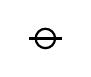
\begin{tikzpicture}[baseline=-0.5ex, line width=0.8pt]
  \draw (0,0) circle (0.35em);
  \draw (-0.6em,0) -- (0.6em,0);
\end{tikzpicture}%
}


\definecolor{DarkBlueContour}{RGB}{0, 0, 150}
\definecolor{LightBlueFill}{RGB}{173, 216, 230}


% --- TikZ & Beamer Overlay Setup ---
% \tikzstyle{point}=[circle, fill=blue, inner sep=2.5pt]
\tikzset{
    alt/.code args={<#1>#2#3}{%
        \alt<#1>{\pgfkeysalso{#2}}{\pgfkeysalso{#3}}%
    },
    highlight/.style args={<#1>}{%
        alt=<#1>{ fill opacity = 1,
            draw opacity = 1
        }{ fill opacity = 0.2, draw opacity = 0.2
        }
    },
    point/.style args={<#1>}{%
        alt=<#1>{ circle,
            fill=blue,
            inner sep=2.5pt
        }{ circle, 
            fill=blue, 
            fill opacity = 0.25, 
            draw opacity = 0.2,
            inner sep = 2.5pt
        }
    },
    pt/.style = {
        circle,
        fill=blue,
        inner sep=2.5pt
    },
    ptfade/.style = {
        circle, 
        fill=blue, 
        fill opacity = 0.25, 
        draw opacity = 0.2,
        inner sep = 2.5pt
    },
    % The style for edges
    edge/.style={
        thick, 
        black!70,
        >=latex,
        opacity=0.3
    },
    vertex/.style = {
        circle,
        draw=DarkBlueContour,
        fill=LightBlueFill,
        minimum size=20pt,
        inner sep=0pt,
        fill opacity=0.3,
        draw opacity = 0.3,
    }
}

\tikzset{
  bnode/.style={
    draw,
    rectangle split,
    rectangle split horizontal,
    rectangle split parts=2,
    text width=0.5cm, 
     align=center,
    minimum width=2cm,
    minimum height=0.8cm,
    inner sep=2pt,
    thick,
    font=\bfseries
  },
  level 1/.style={sibling distance=4cm, level distance=1.8cm},
  level 2/.style={sibling distance=2cm, level distance=1.8cm},
  level 3/.style={sibling distance=1.5cm, level distance=1.8cm},
  edge from parent/.style={
    draw,
    ->,
    thick
  }
}

\title{Arbre KD — KD-Tree}
\subtitle{Étapes de la Construction}
\author{Algorithmes et Pensée Computationnelle \newline \newline  {\small UNIL — École des Sciences Criminelles}}
\date{}


\begin{tikzfadingfrompicture}[name=fade right]
    \shade[left color=transparent!0, right color=transparent!100] 
        (0,0) rectangle (2,2);
\end{tikzfadingfrompicture}

\newcommand{\fadedsepline}{
    \begin{tikzpicture}
        \fill[
            blue!80!black, % Define the line color
            path fading=fade right, % Apply the custom fading
            shading angle=0 % Ensures the fading is applied horizontally
        ] 
        % Coordinates: (x-start, y-start) rectangle (x-end, y-end)
        (0, 0) rectangle (\linewidth, 0.03cm); 
    \end{tikzpicture}
}

% --- define Styles for Points ---
% Style for the main data points (filled blue)
\tikzstyle{data_point}=[circle, fill=blue, inner sep=2.5pt]
% Style for the x-axis projection mark (unfilled blue circle)
\tikzstyle{projection_mark}=[circle, draw=blue, thick, inner sep=2pt, fill=white]
    
\begin{document}

\begin{frame}
\titlepage
\end{frame}


\begin{frame}{Pseudocode de l'algorithme de construction}
\begin{algorithm}[H]
\caption{BuildKDTree($\text{points}, \text{depth}, k$)}
\label{alg:kdtree-build}
\begin{algorithmic}[1]
\If{$\text{points} = \emptyset$}
    \State \textbf{return} $\text{NIL}$
\EndIf
\State $\text{axis} \leftarrow \text{depth} \ \% \ k$ \Comment{Select axis based on current depth}
\State $\text{points} \leftarrow \text{SORT}(\text{points}, \text{key} = \text{axis})$ \Comment{Sort by current axis}
\State $\text{median\_idx} \leftarrow \text{INTEGER}(\text{length}(\text{points}) / 2 )$ \Comment{Index of median list item}
\State $\text{median} \leftarrow \text{KDNode}(\text{points}[\text{median\_idx}]$)
\State $\text{left} \leftarrow \text{points}[1 \ldots \text{median\_idx} - 1]$ \Comment{Left half of the points list}
\State $\text{right} \leftarrow \text{points}[\text{median\_idx} + 1 \ldots \text{length}(\text{points})]$ \Comment{Right half of the points list}
\State $\text{median.left} \leftarrow \text{BuildKDTree}(\text{left}, \text{depth} + 1, k)$
\State $\text{median.right} \leftarrow \text{BuildKDTree}(\text{right}, \text{depth} + 1, k)$
\State \textbf{return} median
\end{algorithmic}
\end{algorithm}
\end{frame}

\begin{frame}{Exemple d'appel}

 \begin{exampleblock}{Remarque}
Dans cet exemple, nous prenons $k$=2 et $points = [(1, 2), (2, 4), (4, 1), (5, 3),$ $(7, 7), (8, 6)]$. Pour rappel, $k$ est la dimension des points dans la liste $points$. 
\end{exampleblock} 
\vspace*{0.5cm}
\fadedsepline
On appelle la fonction BuildKDTree dans le bloc (méthode en Java) \texttt{main} de la manière suivante: BuildKDTree(points, 0, 2) \newline 

On omet \texttt{root} afin de simplifier le dessin de l'arbre. 
    
\end{frame}


\begin{frame}\frametitle{%
    \only<1>{\ \ Répartition de l'espace après le premier appel de BuildKDTree}%
    \only<2>{\ \ Répartition de l'espace après le deuxième appel de BuildKDTree}
    \only<3>{\ Répartition de l'espace après le troisième appel de BuildKDTree}
    \only<4>{Répartition de l'espace après le quatrième appel de BuildKDTree}%
    \only<5>{Répartition de l'espace après le cinquième appel de BuildKDTree}
    \only<6>{\!\!Répartition de l'espace après le sixième appel de BuildKDTree}
}



\begin{minipage}{0.48\textwidth}
        \centering
        \only<1-2>{
            \vspace*{0.25cm}
        }
        \begin{tikzpicture}[scale=0.6]

    % --- 1. Draw the Grid ---
    % The grid extends from (0,0) to (9,8)
    \draw[step=1cm, very thin, gray!50] (0,0) grid (9,8);

    % --- 2. Draw the Axes ---
    % X-axis with arrow and label
    \draw[->, thick] (0,0) -- (9.5,0) node[right] {$x$};
    % Y-axis with arrow and label
    \draw[->, thick] (0,0) -- (0,8.5) node[above] {$y$};

    % --- 3. Add Ticks and Labels to the Axes ---
    % X-axis ticks (from 1 to 9)
    \foreach \x in {1,...,9}
        \draw (\x,0.1) -- (\x,-0.1) node[below] {$\x$};
        
    % Y-axis ticks (from 1 to 8)
    \foreach \y in {1,...,8}
        \draw (0.1,\y) -- (-0.1,\y) node[left] {$\y$};
        
    % Draw the projection
     \only<1>{
        \foreach \x/\y/\lab in {1/2/A, 2/4/B, 4/1/C, 7/7/E, 8/6/F}
        {
            % 3a. Draw the vertical dashed line from the data point to the x-axis
            \draw[dashed, thin, blue!70] (\x, \y) -- (\x, 0);
    
            % 3b. Mark the intersection on the x-axis (unfilled blue circle)
            \node[projection_mark] at (\x, 0) {};
    
            % 3c. Plot the original data point (filled blue circle)
            \node[data_point, label={[label distance=1pt] above right:$\lab$}] at (\x, \y) {};
        }

        % Projection point for the median
        \node[projection_mark, draw=ForestGreen] at (5, 0) {};

        % Median point in Green
        \node[data_point,  label={[label distance=1pt] right:$D$}, fill=ForestGreen] at (5, 3) {};
    }
    % Axis created by the median
    \only<1->{ \draw[dashed, very thick, ForestGreen] (5, 8) -- (5, 0.2); }
    
    \only<2>{
        \fill[blue!20, opacity=0.35] (0, 0) rectangle (5, 8);
        % List of points to plot as faded
        \foreach \x/\y/\lab in {7/7/E, 8/6/F} 
        {
            \node[ptfade] at (\x, \y) {};
            \node[label={[label distance=1pt, text opacity=0.3] above right:$\lab$}] at (\x, \y) {};
        }

        % The previous median faded
        \node[data_point, fill=ForestGreen, fill opacity=0.3, label={[label distance=1pt, text opacity=0.3] above right:$D$}] at (5, 3) {};
            
        \foreach \x/\y/\lab in {2/4/B, 4/1/C}
        {
            % 3a. Draw the vertical dashed line from the data point to the x-axis
            \draw[dashed, thin, blue!70] (\x, \y) -- (0, \y);
    
            % 3b. Mark the intersection on the x-axis (unfilled blue circle)
            \node[projection_mark] at (0, \y) {};
    
            % 3c. Plot the original data point (filled blue circle)
            \node[data_point, label={[label distance=1pt, text opacity=1] above right:$\lab$}] at (\x, \y) {};
        }

        % Projection point for the median
        \node[projection_mark, draw=ForestGreen] at (0, 2) {};

        % Median point in green
        \node[data_point, fill=ForestGreen, label={[label distance=1pt, text opacity=1] above right:$A$}] at (1, 2) {};
    }
    % Axis created by the median
    \only<2->{
        \draw[dashed, very thick, ForestGreen] (5, 2) -- (0.1, 2);
    }
    \only<3>{
        \fill[blue!20, opacity=0.35] (0, 0) rectangle (5, 2);
        % List of points to plot as faded
        \foreach \x/\y/\lab in {2/4/B, 7/7/E, 8/6/F}
        {
            \node[ptfade] at (\x, \y) {};
            \node[label={[label distance=1pt, text opacity=0.3] above right:$\lab$}] at (\x, \y) {};
        }

        % The previous medians faded
        \node[data_point, fill=ForestGreen, fill opacity=0.3, label={[label distance=1pt, text opacity=0.3] above right:$D$}] at (5, 3) {};
        \node[data_point, fill=ForestGreen, fill opacity=0.3, label={[label distance=1pt, text opacity=0.3] above right:$A$}] at (1, 2) {};

        % Projection point for the median
        \node[projection_mark, draw=ForestGreen] at (4, 0) {};

        % Median point in green
        \node[data_point, fill=ForestGreen, label={[label distance=1pt, text opacity=1] above right:$C$}] at (4, 1) {};
    }
    % Axis created by the median
    \only<3->{
        \draw[dashed, very thick, ForestGreen] (4, 2) -- (4, 0.15);
    }



    \only<4>{
        \fill[blue!20, opacity=0.35] (0, 2) rectangle (5, 8);
        % List of points to plot as faded
        \foreach \x/\y/\lab in {7/7/E, 8/6/F}
        {
            \node[ptfade] at (\x, \y) {};
            \node[label={[label distance=1pt, text opacity=0.3] above right:$\lab$}] at (\x, \y) {};
        }


        % The previous medians faded
        \node[data_point, fill=ForestGreen, fill opacity=0.3, label={[label distance=1pt, text opacity=0.3] above right:$D$}] at (5, 3) {};
        \node[data_point, fill=ForestGreen, fill opacity=0.3, label={[label distance=1pt, text opacity=0.3] above right:$A$}] at (1, 2) {};
        \node[data_point, fill=ForestGreen, fill opacity=0.3, label={[label distance=1pt, text opacity=0.3] above right:$C$}] at (4, 1) {};

        % Projection point for the median
        \node[projection_mark, draw=ForestGreen] at (2, 0) {};

        % Median point in green
        \node[data_point, fill=ForestGreen, label={[label distance=1pt, text opacity=0.9] above right:$B$}] at (2, 4) {};
    }
    % Axis created by the median
    \only<4->{
        \draw[dashed, very thick, ForestGreen] (2, 2) -- (2, 8);
    }

    
     \only<5>{
        \fill[blue!20, opacity=0.35] (5, 0) rectangle (9, 8);
        
        \node[data_point, label={[label distance=1pt, text opacity=1] above right:$F$}] at (8, 6) {};
         
        % The previous medians faded
        \node[data_point, fill=ForestGreen, fill opacity=0.3, label={[label distance=1pt, text opacity=0.3] above right:$D$}] at (5, 3) {};
        \node[data_point, fill=ForestGreen, fill opacity=0.3, label={[label distance=1pt, text opacity=0.3] above right:$A$}] at (1, 2) {};
        \node[data_point, fill=ForestGreen, fill opacity=0.3, label={[label distance=1pt, text opacity=0.3] above right:$C$}] at (4, 1) {};
        \node[data_point, fill=ForestGreen, fill opacity=0.3, label={[label distance=1pt, text opacity=0.3] above right:$B$}] at (2, 4) {};

        % Projection point for the median
        \node[projection_mark, draw=ForestGreen] at (0, 7) {};
        \node[projection_mark, draw=blue] at (0, 6) {};

        % Median point in green
        \node[data_point, fill=ForestGreen, label={[label distance=1pt, text opacity=1] above right:$E$}] at (7, 7) {};
    }
    % Axis created by the median
    \only<5->{
        \draw[dashed, very thick, ForestGreen] (5, 7) -- (9, 7);
    }



    \only<6>{
        %  Last region to shade
        \fill[blue!20, opacity=0.35] (5, 0) rectangle (9, 7);
        
        \node[data_point] at (8, 6) {};
         
        % The previous medians faded
        \node[data_point, fill=ForestGreen, fill opacity=0.3, label={[label distance=1pt, text opacity=0.3] above right:$D$}] at (5, 3) {};
        \node[data_point, fill=ForestGreen, fill opacity=0.3, label={[label distance=1pt, text opacity=0.3] above right:$A$}] at (1, 2) {};
        \node[data_point, fill=ForestGreen, fill opacity=0.3, label={[label distance=1pt, text opacity=0.3] above right:$C$}] at (4, 1) {};
        \node[data_point, fill=ForestGreen, fill opacity=0.3, label={[label distance=1pt, text opacity=0.3] above right:$B$}] at (2, 4) {};
        \node[data_point, fill=ForestGreen, fill opacity=0.3, label={[label distance=1pt, text opacity=0.3] above right:$E$}] at (7, 7) {};

        % Projection point for the median
        \node[projection_mark, draw=ForestGreen] at (8, 0) {};

        % Median point in green
        \node[data_point, fill=ForestGreen, label={[label distance=1pt, text opacity=0.3] above right:$F$}] at (8, 6) {};
    }
    % Axis created by the median
    \only<6->{
        \draw[dashed, very thick, ForestGreen] (8, 0.13) -- (8, 7);
    }

\end{tikzpicture}
\end{minipage}
\hspace*{0.1cm}
\begin{minipage}{0.40\textwidth}
    \centering
    \only<1-2>{
            \vspace*{0.25cm}
        }
    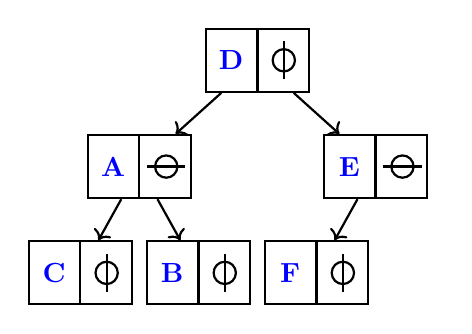
\begin{tikzpicture}[scale=0.75]
  % Tree
  \node[bnode] (n1) {\textcolor{blue}{D}\nodepart{two}{$\vertcirc$}}
    child[highlight=<2->] { 
        node[bnode, highlight=<2->] (n2) {
            \textcolor{blue}{A}\nodepart{two}{$\horcirc$}   
        }
      child[highlight=<3->] { node[bnode, highlight=<3->] (n4) {\textcolor{blue}{C}\nodepart{two}{$\vertcirc$}} }
      child[highlight=<4->] { node[bnode, highlight=<4->] (n5) {\textcolor{blue}{B}\nodepart{two}{$\vertcirc$}}
      }
    }
    child[highlight=<5->] { node[bnode, highlight=<5->] (n3) {\textcolor{blue}{E}\nodepart{two}{$\horcirc$}}
      child[highlight=<6->] { node[bnode, highlight=<6->] (n7) {\textcolor{blue}{F}\nodepart{two}{$\vertcirc$}}
      }
     child[edge from parent path={}] { node { } }
    };

\end{tikzpicture}
\end{minipage}


    


\begin{itemize}
    \item<2-> \only<2>{On considère les points dans la région $x \leq 5$ càd $[C, A, B]$}   
    \only<3>{On considère les points dans la région $x \leq 5$ et $y\leq 2$ càd $[C]$}   
    \only<4>{On considère les points dans la région $x \leq 5$ et $y>2$ càd $[B]$}   
    \only<5>{On considère les points dans la région $x > 5$ càd $[F, E]$}   
    \only<6>{On considère les points dans la région $x > 5$ et $y \leq 7$ càd $[F]$}   

    
    \item<1-> \only<1>{Le point milieu (median) en vert est à l'indice 3 dans la liste $points$ triée selon le premier axe (horizontal).} 
    \only<2>{Le point milieu est à l'indice 1 dans la liste triée selon le deuxième axe (vertical).}  
    \only<3>{Le point milieu est à l'indice 0 car il n'y a pas d'autres points.}
    \only<4>{Le point milieu est à l'indice 0 car il n'y a pas d'autres points.}
    \only<5>{Le point milieu est à l'indice 1 car il y a deux points.}
    \only<6>{Le point milieu est à l'indice 0 car il n'y a pas d'autres points.}
    
\end{itemize}
\end{frame}




\end{document}